\section{Zielsetzung}
Bei diesem Versuch soll die Halbwertszeit zweier verschiedener Elemente mittels
Aktivierung mit Neutronen untersucht werden.

\section{Theorie}
Der Zerfall radioaktiver Isotope beruht darauf, dass das Verhältniss von Neutronen
und Protonen außerhalb eines bestimmten Bereiches liegt und die Kerne somit instabil
werden.
Die Halbwertszeiten T, also die Zeiten, in denen etwa die Hälfte der Kerne des vorliegenden
Materials zerfallen sind, liegt bei den hier verwendeten Isotopen im Bereich von einigen
Sekunden bis Stunden. Daher müssen die instabilen Isotope, welche untersucht werden
sollen, erst kurz vor dem Versuch erzeugt werden. \\
Zu diesem Zweck werden stabile Kerne mit freien Neutronen bestrahlt, welche
aufgrund der neutralen Ladung die Coulomb-Barriere nicht überwinden müssen und somit leichter
in den Kern eindringen können.
Gelangt ein Neutron in einen Kern A, so entsteht zunächst ein sogenannter Zwischenkern
oder auch Compoundkern $\text{A}^*$, welcher aufgrund der kinetischen Energie und
der Bindungsenergie des Neutrons energetisch höher liegt als der Kern A.
Die zusätzliche Energie wird allerdings sehr schnell auf alle Nukleonen verteilt, sodass
das Neutron nicht direkt wieder abgestrahlt werden kann. Stattdessen geht der
Compoundkern unter Emission eines $\gamma$-Quants nach etwa ${10^{-16}}\si{\second}$
in seinen Grundzustand über, sodass insgesamt die Reaktion
\begin{equation}
  \ce{^{m}_{z}A + ^1_0n -> ^{m+1}_{z}A^* -> ^{m+1}_{z}A} + \gamma
  \label{eqn:reak1}
\end{equation}
abläuft.
Da nun bei dem neu entstandenen Kern das Verhältniss von Protonen und Neutronen außerhalb
des stabilen Bereichs liegt, ist der so entstandene Kern instabil. Er wandelt sich
durch einen $\beta$-Zerfall, also unter Emission eines Elektrons und eines Antineutrinos
in einen neuen stabilen Kern C um. Die Reaktionsgleichung lautet:
\begin{equation}
  \ce{^{m+1}_{z}A -> ^{m+1}_{z+1}C} + \beta^- + \text{E}_{\text{kin}} + \bar{\nu}_e
  \label{eqn:reak2}
\end{equation}
\\
Um die Wahrscheinlichkeit eines Neutroneneinfangs anzugeben wird der Wirkungsquerschnitt
mit der Gleichung
\begin{equation}
  \sigma = \frac{\text{u}}{\text{n}\text{K}\text{d}}
  \label{eqn:wqs}
\end{equation}
eingeführt, welcher so definiert ist, dass bei einem Beschuss von n Neutronen pro
Sekunde auf eine dünne Folie mit Dicke d und K Atomen pro Kubikcentimeter u Einfänge
stattfinden. Somit ist die Einheit des Wirkungsquerschnitt durch ${10^{-24}}\si{\square\centi\meter}$
=: 1barn gegeben.\\
Hierbei ist der Wirkungsquerschnitt antiproportional zur Geschwindigkeit der Neutronen, es
gilt also
\begin{equation}
  \sigma \propto \frac{1}{\text{v}} \: .
  \label{eqn:antiprop}
\end{equation}
Dies lässt sich anschaulich darüber erklären, dass sich langsame Neutronen länger in der
Nähe eines Kerns aufhalten und somit die Wahrscheinlichkeit eines Einfangens steigt.
Es kann zudem zu Resonanzeffekten kommen, falls die Energie des Neutrons genau
die Energiedifferenz zweier Anregungszustände des Zwischenkerns trifft. \\
Da freie Neutronen allerdings nur eine Halbwertszeit von etwa 15 Minuten besitzen und
somit recht schnell zerfallen, müssen auch die zur Aktivierung benötigten Neutronen
zunächst vor dem Experiment erzeugt werden.
Dies erfolgt über die Bestrahlung von Beryllium mit $\alpha$-Teilchen aus dem
Zerfall von $\ce{^{226}_{88}Ra}$, wobei die Reaktion
\begin{equation}
  \ce{^{9}_{a}Be + ^{4}_{2}}\alpha \ce{-> ^{12}_{6}C + ^1_0n}
\end{equation}
abläuft.\\
Da die Neutronen aufgrund des kontinuierlichen Energiespektrums teilweise sehr hohe
Energien von bis zu $\SI{13.7}{\mega\electronvolt}$ besitzen, müssen sie zunächst
noch abgebremst werden um die bereits erwähnte, möglichst geringe Geschwindigkeit zu
erreichen.
Dazu werden die Neutronen in eine dicke Schicht aus Atomen mit möglichst
leichten Kernen geleitet, da dabei durch elastische Stöße eine hohe Energieübertragung stattfindet.
In diesem Aufbau wird dazu Paraffin verwendet, wie in Abbildung
\ref{fig:neut} zu sehen ist, da es einen hohen Anteil an Wasserstoff-Atomen besitzt.
\begin{figure}[H]
  \centering
  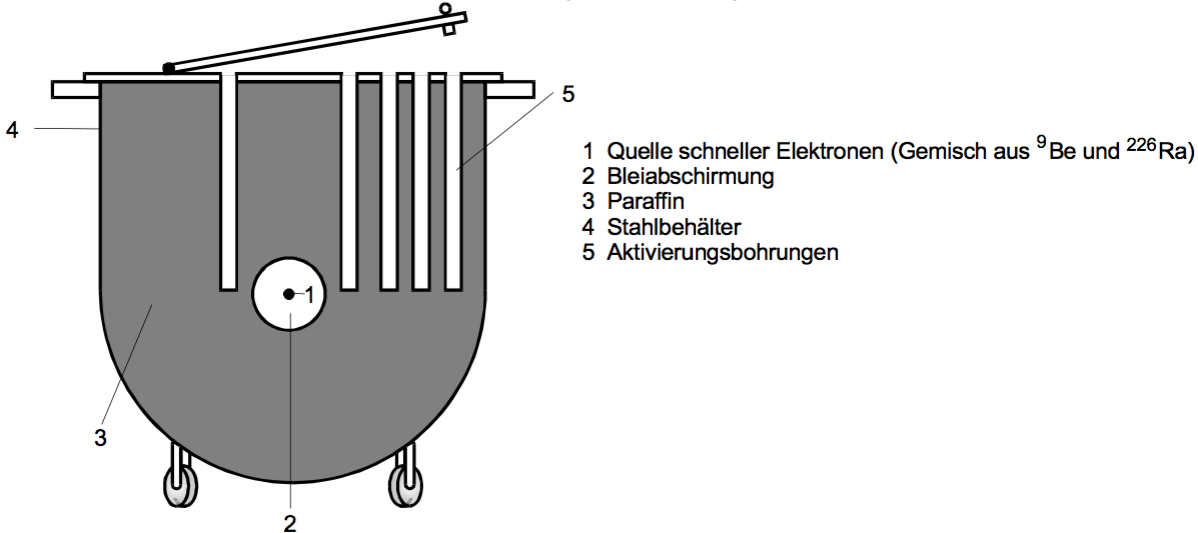
\includegraphics[height=5cm]{Neutron.png}
  \caption{Skizzierter Querschnitt der Neutronenquelle \cite{skript}.}
  \label{fig:neut}
\end{figure}
Anschließend haben die Neutronen eine mittlere Geschwindigkeit von etwa $\SI{2.2}{\kilo\meter\per\second}$
und werden als thermische Neutronen bezeichnet. \\
Bei diesem Versuch wird die Aktivierung der stabilen Isotope
$\ce{^{115}_{49}In}$, $\ce{^{107}_{47}Ag}$ und $\ce{^{109}_{47}Ag}$
und der anschließende Zerfalls der somit neu enstandenen Isotope untersucht.
Die Reaktionsgleichungen lauten hierbei:
\begin{align}
  \ce{^{115}_{49}In + ^1_0n -> ^{116}_{49}In -> ^{116}_{50}Sn} + \beta^- + \bar{\nu}_e \\
  \ce{^{107}_{47}Ag + ^1_0n -> ^{108}_{47}Ag -> ^{108}_{48}Cd} + \beta^- + \bar{\nu}_e \\
  \ce{^{109}_{47}Ag + ^1_0n -> ^{110}_{47}Ag -> ^{110}_{48}Cd} + \beta^- + \bar{\nu}_e
\end{align}
Der $\beta^-$-Zerfall der instabilen Isotope verläuft dabei gemäß der Gesetzmäßigkeit des radioaktiven
Zerfalles, bei welchen die Anzahl N der zum Zeitpunkt t noch nicht zerfallenen
Kerne durch
\begin{equation}
  \text{N}(\text{t}) = \text{N}_0 \text{e}^{ -\lambda \text{t}}
  \label{eqn:zerfall}
\end{equation}
gegeben ist, wobei $\text{N}_0$ die Anfangszahl der radioaktivien Kerne bezeichnet und
$\lambda$ die Zerfallskonstante, welche durch die Gleichung
\begin{equation}
  \text{T} = \frac{\ln{2}}{\lambda}
  \label{eqn:zkonst}
\end{equation}
mit der Halbwertszeit T verknüpft ist. \\
Da die direkte Messung von $\text{N}(\text{t})$ jedoch sehr schwierig ist, werden bei diesem
Versuch die Anzahl der in einem bestimmten Zeitintervall $\increment\text{t}$ zerfallenden
Kerne $\text{N}_{\increment\text{t}}$ verwendet, welche sich leicht durch beispielsweise
ein Geiger-Müller-Zählrohr messen lassen.
Diese Anzahl ist gegeben durch
\begin{equation}
  \text{N}_{\increment\text{t}} = \text{N}(\text{t}) -\text{N}(\text{t} + \increment \text{t}) \:,
  \label{eqn:dN}
\end{equation}
woraus sich durch die Formel \ref{eqn:zerfall} die Gleichung
\begin{equation}
  \text{N}_{\increment\text{t}} =\text{N}_0 \text{e}^{ -\lambda \text{t}} - \text{N}_0 \text{e}^{ -\lambda (\text{t}+\increment \text{t})}
  = \text{N}_0 (1- \text{e}^{ -\lambda \increment \text{t}})\text{e}^{ -\lambda \text{t}}
  \label{eqn:N}
\end{equation}
ergibt, und somit also auch
\begin{equation}
  \ln{\text{N}_{\increment\text{t}}} = \ln{\text{N}_0(1-\text{e}^{ -\lambda \increment \text{t}})} -\lambda \text{t} \:.
  \label{eqn:lnN}
\end{equation}
\\
Wichtig ist es dabei ein geeignetes Zeitintervall $\increment\text{t}$ zu wählen, um sowohl
den statistischen Fehler von $\text{N}_{\increment\text{t}}$ aufgrund von zu kleinen
$\increment\text{t}$ als auch den systematischen Fehler von $\lambda$ durch zu groß gewählte
$\increment\text{t}$ gering zu halten.\\
Zudem ist bei der Messung von Silber zu beachten, dass das natürliche Silber stets
aus einem Gemisch aus etwa 51,8\% des Isotops $\ce{^{107}_{47}Ag}$ und etwa 48,2\% $\ce{^{109}_{47}Ag}$
besteht, sodass zunächst die Zerfallsreaktionen von $\ce{^{108}_{47}Ag}$ und $\ce{^{110}_{47}Ag}$
parallel zueinander ablaufen und sich bei der Messung nicht unterscheiden lassen.
Da das Isotop $\ce{^{110}_{47}Ag}$ jedoch eine kürzere Halbwertszeit besitzt,
ist dieser Anteil nach einer gewissen Zeit $\text{t}^*$, welche selbst aus dem Graphen festgelegt wird,
praktisch fast vollständig zerfallen.
Die gemessene Aktivität rührt ab da zu einem großen Teil nur noch vom langlebigeren Isotop
$\ce{^{108}_{47}Ag}$ her.
Für größere Zeiten als dieses $\text{t}^*$ lässt sich im Zerfalls-Diagramm, welches in
Abbildung \ref{fig:abfall} dargestellt ist, eine Gerade erkennen, sodass sich mit diesen
Wertepaaren durch eine lineare Ausgleichsrechnung die Zerfallskonstante $\lambda_l$
des langlebigeren $\ce{^{108}_{47}Ag}$ bestimmen lässt, wobei die Zerfallsgleichung damit
\begin{equation}
  \text{N}_l(\text{t}) = \text{N}_{0l} \text{e}^{ -\lambda_l \text{t}}
  \label{eqn:zl}
\end{equation}
lautet.

Zur Bestimmung der kleineren Zerfallskonstante $\lambda_k$ werden von den insgesamt gemessenen
Werten $\text{N}_{\increment\text{t}}$
zunächst die Werte
\begin{equation}
  \text{N}_{\increment\text{t}l} = \text{N}_{0l} (1- \text{e}^{ -\lambda_l \increment \text{t}})\text{e}^{ -\lambda_l \text{t}}
\end{equation}
subtrahiert, und anschließend mit der Differenz eine lineare Ausgleichsrechnung durchgeführt,
jedoch nur für Zeiten kleiner als ein Zeitpunkt $\text{t}_i$ mit
$\text{t}_i < \text{t}^*$, sodass die statistischen Schwankungen nicht zu groß werden.
\begin{figure}[H]
  \centering
  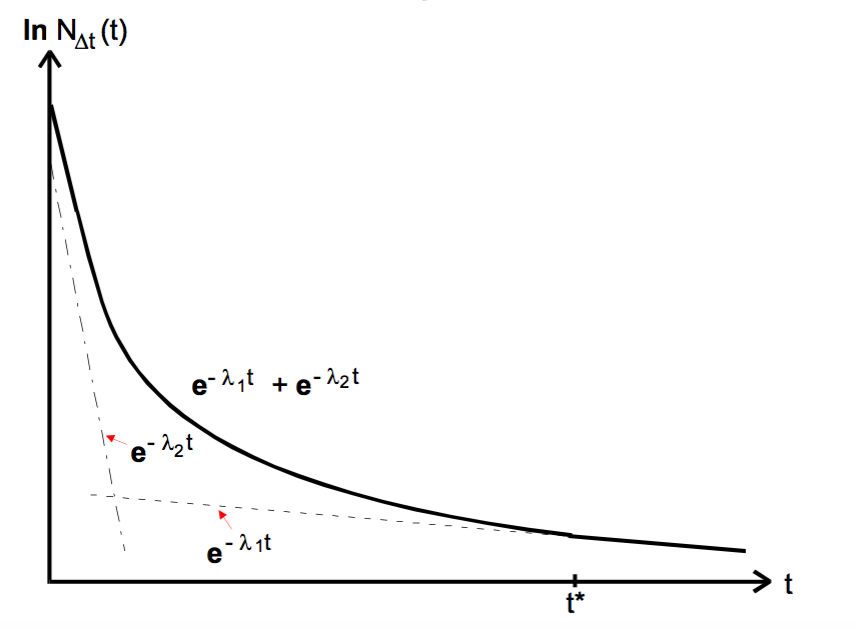
\includegraphics[height=5cm]{Abfall.png}
  \caption{Skizzierter Querschnitt der Neutronenquelle \cite{skript}.}
  \label{fig:abfall}
\end{figure}
